\documentclass[mathserif]{beamer}
\usepackage{graphicx}
\usepackage{tikz}
\usepackage{multicol}

\begin{document}
\title{Title}
\author{Akshay Sanjeev, Hitesh, Janani}

\begin{frame}
    \maketitle
\end{frame}

\begin{frame}{Acousitc Localization vs Echo-lcoation}

\end{frame}
\begin{frame}{Acoustic localisation on a line}
    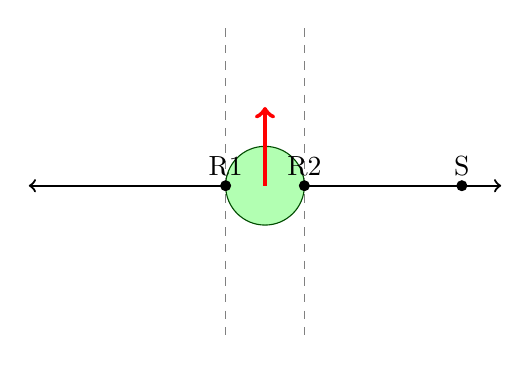
\begin{tikzpicture}
        \
        % Midpoint of the line
        \coordinate (M) at (0,0);
        \coordinate (R1) at (-0.5,0);
        \coordinate (R2) at (0.5,0);

        \coordinate (S) at (2.5,0);
        \draw[thick,<->] (-3,0) -- (3,0);
        \draw[fill=green!30, draw=green!30!black] (M) circle[radius=0.5];
        \draw[line width=1.6pt,color=red, ->] (0, 0) -- (0, 1);
        \draw[dashed, color= gray] (-.5, 2) -- (-.5,-2);
        \draw[dashed, color= gray] (.5, 2) -- (.5,-2);

        \fill (R1) circle (2pt) node[above] {R1};
        \fill (R2) circle (2pt) node[above] {R2};
        \fill (S)  circle (2pt) node[above] {S};
        % Network architecture

        % \coordinate (I) at (0, -2);
        % \draw[fill = yellow!30] (I) circle[radius=.25];
        % \draw[thick, ->] (-.5, 0) -- (0, -2);%R1->I
        % \draw[thick, ->] ( .5, 0) -- (0, -2);%R2-I

        % \coordinate (O1) at ()

    \end{tikzpicture}
\end{frame}
\begin{frame}
    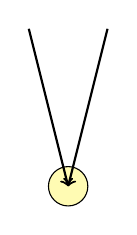
\begin{tikzpicture}
            \coordinate (I) at (0, -2);
        \draw[fill = yellow!30] (I) circle[radius=.25];
        \draw[thick, ->] (-.5, 0) -- (0, -2);%R1->I
        \draw[thick, ->] ( .5, 0) -- (0, -2);%R2-I
    \end{tikzpicture}
\end{frame}


\begin{frame}{Acoustic localisation on a plane}
    
\end{frame}
\end{document}